\chapter{Deep Learning Models for Carbohydrate and Bolus Recommendations}
\label{chapter:models}

This chapter will expand on the general problem description from Section~\ref{section:objective} and introduce in detail the situations commonly encountered in diabetes self-management that could benefit from the research reported in this thesis. Two neural network models will be introduced, as well as a two baseline models, and all will be evaluated extensively on the tasks of carbohydrate and bolus recommendation using examples extracted from the OhioT1DM dataset.

\section{Recommendation Scenarios}
\label{sec:scenarios}

It is assumed that blood glucose levels are measured at 5 minute intervals through a \ac{CGM} system. It is also assumed that discrete deliveries of insulin (boluses) and continuous infusions of insulin (basal rates) are recorded. Subjects provide the timing of meals and estimates of the number of grams of carbohydrate in each meal. Given the available data up to and including the present (time $t$), the system aims to estimate how much a person should eat or bolus 10 minutes from now (time $t+10$) such that their blood glucose will reach a target level $\tau$ minutes after that action (time $t + 10 + \tau$). A system that computes these estimates could then be used in the following three recommendation scenarios:
\begin{enumerate}
    \item {\bf Carbohydrate Recommendations}: Estimate the amount of carbohydrate $C_{t+10}$ to have in a meal in order to achieve a target \ac{BG} value $G_{t+10+\tau}$.
    \item {\bf Bolus Recommendations}: Estimate the amount of insulin $B_{t+10}$ to deliver with a bolus in order to achieve a target \ac{BG} value $G_{t+10+\tau}$.
    \item {\bf Bolus Recommendations given Carbohydrates}: Expecting that a meal with $C_{t+20}$ grams of carbohydrate will be consumed 20 minutes from now, estimate the amount of insulin $B_{t+10}$ to deliver with a bolus 10 minutes before the meal in order to achieve a target \ac{BG} value $G_{t+10+\tau}$.
\end{enumerate}
These recommendation scenarios were designed to align with decision-making situations commonly encountered by people with type 1 diabetes. In particular, the corresponding recommendation systems would help an individual to estimate how much to eat or bolus for the purpose of raising or lowering their \ac{BGL} (scenarios 1 and 2), as well as how much to bolus for a planned meal (scenario 3). 

%\textcolor{blue}{While all three of these scenarios are useful, there are two specific subsets of these cases that are of particular interest. The carbohydrate recommendation scenario evaluated only on meals that do not have an associated boluses is especially relevant because these are the situations where a subject presumably ate a snack specifically to raise their BGL. The bolus recommendation scenario trained and evaluated exclusively on inertial examples also is particularly useful, as the boluses in these examples are not taken with a meal. This means that these boluses were likely taken to lower the subject's BGL. These two specific scenarios are the most interesting in practice. However, they both are fairly uncommon in the particular dataset that we used.}

%In the following Section~\ref{sec:models}, \textcolor{blue}{a number of baseline models and neural architectures are described}, all implementing the three types of recommendations. The neural architectures use Long Short-Term Memory (LSTM) networks either in a standalone prediction model (Section~\ref{sec:lstm}) or integrated as basic repeating blocks in a deep residual network (Section~\ref{sec:nbeats}). The models are trained on examples extracted from the OhioT1DM dataset~\cite{ohiot1dm:marling:kdh18}, as explained in Chapter~\ref{chapter:data}. Ideally, to match the intended use of these recommendations in practice, training examples should not have any extra meals or boluses in the prediction window $[t, t + 10 + \tau]$. Following the terminology from \cite{mirshekarian:bgl_pred}, \textcolor{blue}{these examples are called {\it inertial} examples.} However, to benefit from a larger number of training examples, \textcolor{blue}{models are also trained and evaluated on a more general class of {\it unrestricted} examples}, in which other bolus or meal events are allowed to appear in the prediction window. Correspondingly, experimental results for inertial vs. unrestricted examples are presented in Section~\ref{sec:results}. 

%The paper ends in Section~\ref{sec:conclusion} with concluding remarks and ideas for future work.
% In Section~\ref{sec:results} we show the extent to which models trained on the larger set of unrestricted examples transfer to inertial examples.

%Ideally, all examples of the above prediction scenarios in the data would not have any extra meals or boluses in the prediction window between $t$ and $t+10+\tau$. These events would not be known in practice since they are in the future. However, if only examples without these such events were used, it would limit the number of examples that can be extracted from the data. For this reason, examples are separated into 2 classes based on the following criteria:

%\begin{enumerate}
%    \item {\bf Class $\mathbf{C_{1}}$} examples do not contain events in the prediction window $(t, t+10+\tau)$ other than the meal or bolus that is to be predicted. When the bolus given carbohydrates prediction scenario is used, the meal that follows the bolus is also allowed in a C$_1$ example. This class of example most closely represents the situations in which the system would be used in practice. However, these examples are somewhat limited, especially for the bolus prediction scenario.
%    \item {\bf Class $\mathbf{C_{2}}$} is more general and allows other events to be in the prediction window $(t, t+10+\tau)$. This class yields a higher number of examples, but resembles a real world situation less than C$_1$, since there are unknown events past the present time $t$. Because of this, a more complex model is required to process C$_2$ examples.
%\end{enumerate}

%Using both classes of examples allows us to see how well the models do on examples similar to real world use, C$_1$, as well as how well the models do with the maximum number of possible examples in the dataset with C$_2$.


\section{Recommendation Models}
\label{sec:models}

In the following sections, a number of baseline models and neural architectures are described, all implementing the three types of recommendations. The neural architectures use \ac{LSTM} networks either in a standalone prediction model (Section~\ref{sec:lstm}) or integrated as basic repeating blocks in a deep residual network (Section~\ref{sec:nbeats}). The models are trained on examples extracted from the OhioT1DM dataset~\cite{ohiot1dm:marling:kdh18}, as explained in Chapter~\ref{chapter:data}. Ideally, to match the intended use of the recommendation scenarios from Section~\ref{sec:scenarios}, training examples should not have any extra meals or boluses in the prediction window $[t, t + 10 + \tau]$. Following the terminology from \cite{mirshekarian:bgl_pred}, these examples are called {\it inertial} examples. However, to benefit from a larger number of training examples, models are also trained and evaluated on a more general class of {\it unrestricted} examples, in which other bolus or meal events are allowed to appear in the prediction window. Correspondingly, experimental results for both inertial vs. unrestricted examples are presented in Section~\ref{sec:results}.

\subsection{Baseline Models}
Given training data containing time series of blood glucose levels, meals with their carbohydrate intake, and boluses with their corresponding insulin dosages, two baselines are defined as follows:
\begin{enumerate}
    \item {\bf Global average}: 
    For the carbohydrate recommendation scenario, the average number $\mu$ of carbs over all of the meals in the subject's training data is computed and used as the estimate for all future predictions for that subject, irrespective of the context of the example. Analogously, for the bolus and bolus given carbs recommendation scenarios, $\mu$ is the average amount of insulin dosage over all boluses in the subject's training data. This is a fairly simple baseline, as it predicts the same average value for every test example for a particular subject.
    
    %Compute the average number of carbs over all of the meals in the subject's training data, and use this average $\mu$ as the estimate for all future meals, irrespective of context. This is a fairly simple baseline, as it predicts the same value for every example.
    \item {\bf \ac{ToD} average}: In this \ac{ToD} dependent baseline, an average number of carbs or an average amount of bolus insulin is computed for each of the following five time windows during a day:
	\begin{itemize}
		\item 12am-6am: $\mu_1$ = early breakfast / late snacks.
		\item 6am-10am: $\mu_2$ = breakfast.
		\item 10am-2pm: $\mu_3$ = lunch.
		\item 2pm-6pm: $\mu_4$ = dinner.
		\item 6pm-12am: $\mu_5$ = late dinner / post-dinner snacks.
	\end{itemize}
    The average for each \ac{ToD} interval is calculated over all of the meals or boluses appearing in the corresponding time frame in the subject's training data. At test time, to make a recommendation for time $t+10$, the \ac{ToD} interval that contains $t+10$ is determined and the corresponding \ac{ToD} average is used as the recommendation.
\end{enumerate}
Given sufficient historical data, the \ac{ToD} baseline is expected to perform well for individuals who tend to eat very consistently and have regular diets. However, it is expected to perform poorly for individuals who have a lot of variation in their diets.

% For the bolus given carbs recommendation scenario, one might have also considered a bolus calculator `baseline', for which insulin dosages would be computed using the actual bolus calculator employed by the subjects in the OhioT1DM dataset every time they had a meal. However, assuming subjects had perfect adherence to using the bolus calculator, this `baseline' would coincide with the ground truth every time, making it inappropriate as a baseline.

\begin{figure*}[t]
    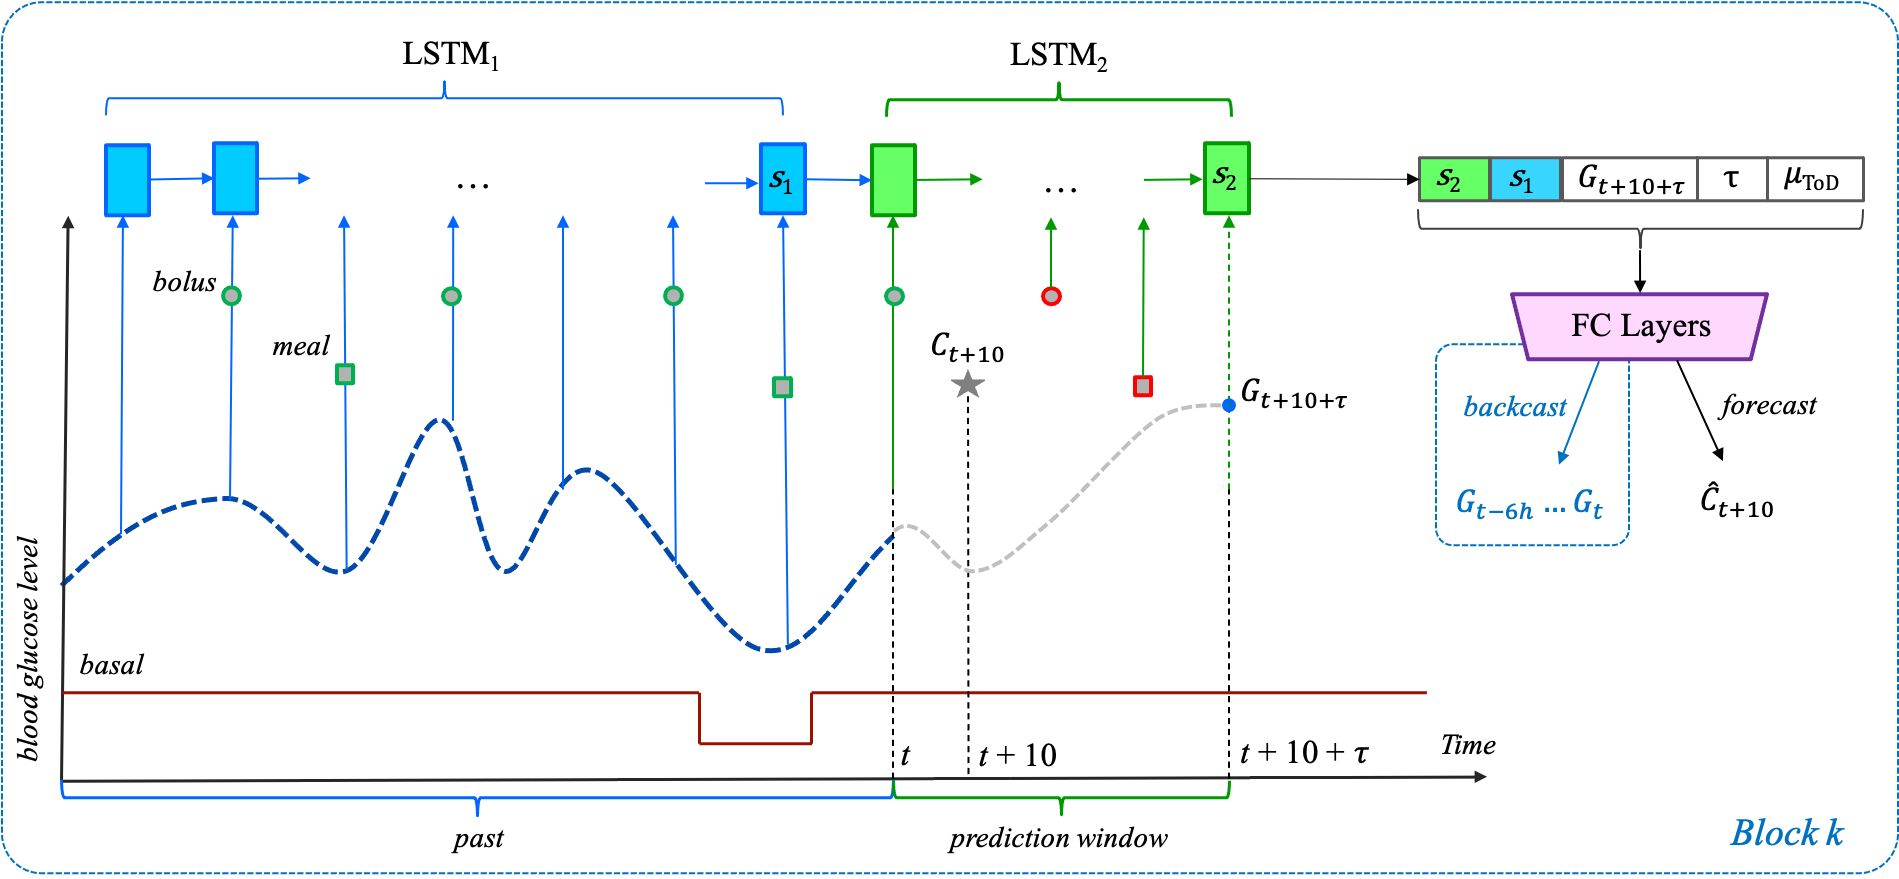
\includegraphics[width=\textwidth]{carbs-block}
    \caption{The general neural network architecture for the carbohydrate recommendation scenario. The dashed blue line in the graph represents a subject's \ac{BGL}, while the solid brown line represents the basal rate of insulin. The gray star represents the meal at time $t+10$. The other meals are represented by squares, and boluses are represented by circles. Meals and boluses with a red outline cannot appear in {\it inertial} examples, but are allowed in {\it unrestricted} examples. The blue units in $\text{LSTM}_{1}$ receive input from different time steps in the past. The green units in $\text{LSTM}_{2}$ receive input from the prediction window. The purple trapezoid represents the 5 fully connected layers, whereas the output node at the end computes the prediction.}
    \label{fig:carbs}
\end{figure*}

\begin{figure*}[t]
    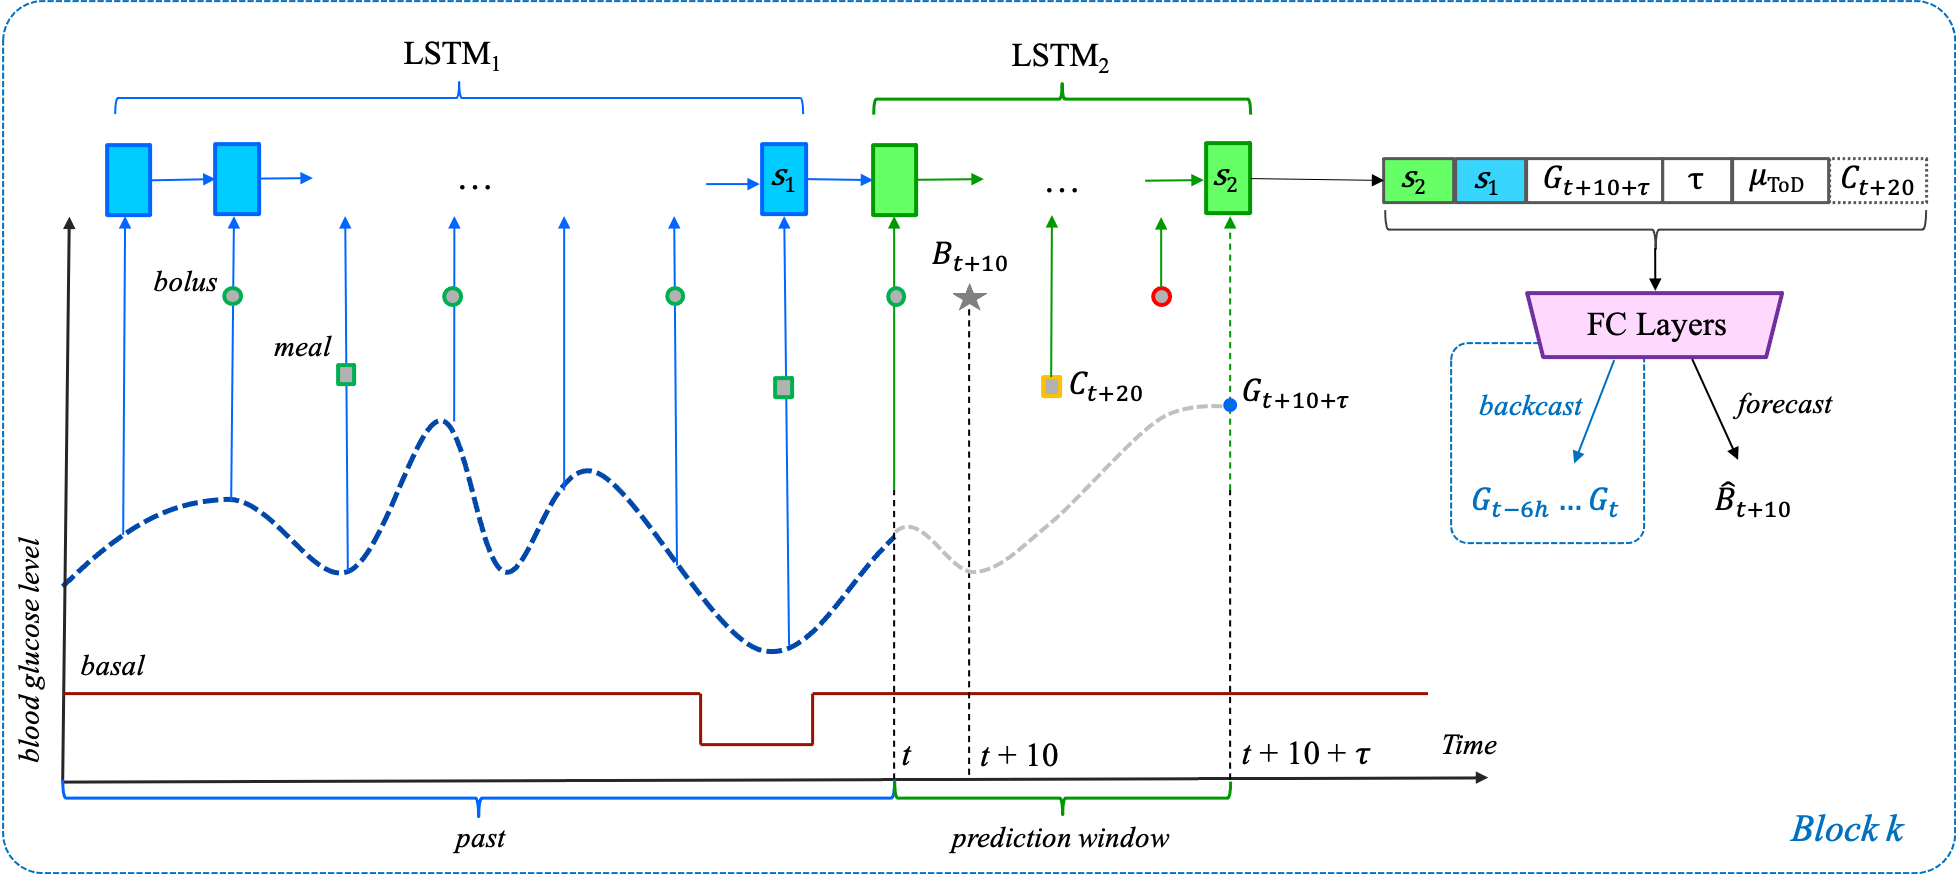
\includegraphics[width=\textwidth]{bolus-block}
    \caption{The general neural network architecture for the bolus and bolus given carbs recommendation scenarios. The architecture itself is similar to that shown in Figure~\ref{fig:carbs}. The gray star now represents the bolus at time $t+10$. For the bolus recommendation scenario, the events outlined in red or orange are not allowed in {\it inertial} examples.  However, in the bolus given carbs scenario, the meal event $C_{t+20}$ shown with the yellow outline is an important part of each example, be it inertial or unrestricted. As such, in this scenario, the dashed $C_{t+20}$ becomes part of the input to the FCN.}
    \label{fig:bolus}
\end{figure*}

\begin{figure*}[t]
    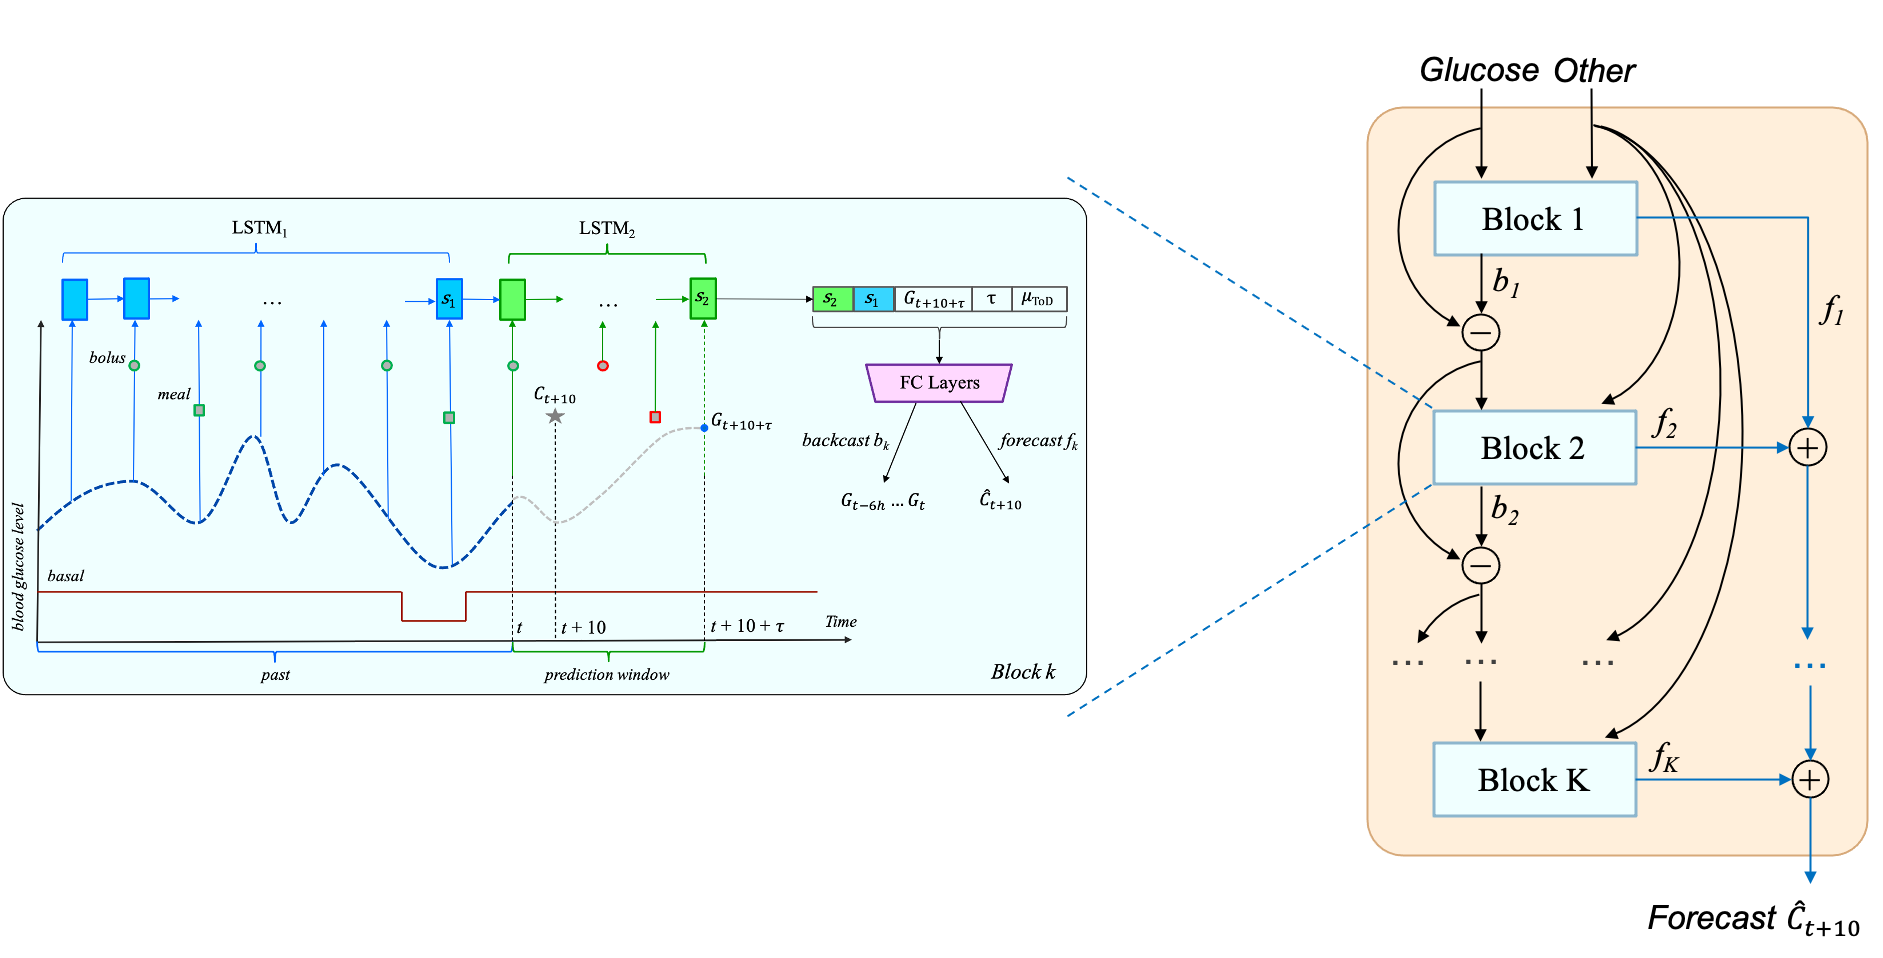
\includegraphics[width=\textwidth]{carbs-nbeats}
    \caption{The N-BEATS inspired deep residual architecture for carbohydrate recommendation. A similar architecture is used for bolus and bolus given carbs recommendations.}
    \label{fig:nbeats}
\end{figure*}


\subsection{LSTM Architectures}
\label{sec:lstm}

While simple to compute and use at test time, the two baselines are likely to give suboptimal performance, as their predictions ignore the history of \ac{BGL} values, insulin (boluses and basal rates), and meals, all of which could significantly modulate the effect a future meal and/or bolus might have on the \ac{BGL}. To utilize this information, the general \ac{LSTM}-based network architectures shown in Figure~\ref{fig:carbs} for carb recommendation and Figure~\ref{fig:bolus} for bolus recommendation were developed. The first component in each architecture is a recurrent neural network instantiated using \ac{LSTM} cells \cite{hochreiter:nc97}, which is run over the previous 6 hours of data, up to and including the present time $t$. At each time step (every 5 minutes), this LSTM$_1$ network takes as input the \ac{BGL}, the carbs, and the insulin dosages recorded at that time step. While sufficient for processing {\it inertial} examples, the same \ac{LSTM} cannot be used to process events that may appear in the prediction window $(t, t+10+\tau)$ of {\it unrestricted} examples, because \ac{BGL} values are not available in the future. Therefore, when training on unrestricted examples, the final state computed by the LSTM$_1$ model at time $t$ is projected using a linear transformation and used as the initial state for a second \ac{LSTM} network, LSTM$_2$, that is run over all the time steps in the prediction window $(t, t+10+\tau)$. The final state computed by LSTM$_1$ (for inertial examples) is appended to the final state computed by LSTM$_2$ (for unrestricted examples) and is then used as input to a \ac{FCN} whose output node computes an estimate of the carbs or bolus insulin at time $t+10$. In addition to the \ac{LSTM} final state(s), the input to the \ac{N-BEATS} contains the following features:
\begin{itemize}
    \item The target blood glucose level $\tau+10$ minutes into the future, i.e., $G_{t + 10 + \tau}$.
    \item The prediction horizon $\tau$.
    \item The \ac{ToD} average for the time frame that contains $t+10$.
    \item For the bolus given carbs scenario only, the planned amount $C_{t + 20}$ of carbohydrate becomes part of the input, too.
\end{itemize}
Each \ac{LSTM} uses vectors of size 32 for the states and gates, whereas the \ac{N-BEATS} is built with up to 5 hidden layers, each consisting of 64 ReLU neurons, and one linear output node. Note that by using the final state of LSTM$_1$  to initialize LSTM$_2$, the latter's final state should theoretically be able to capture any useful information that is represented in the final state of LSTM$_1$, which may call into question the utility of concatenating the two final states. This architectural decision is nevertheless supported empirically through evaluations on the validation data, which show improvements in prediction performance when both states are used (Section~\ref{sec:development}).

\subsection{Deep Residual Networks}
\label{sec:nbeats}

%\citet{oreshkin:nbeats} have recently introduced a new architecture for time series forecasting, the Neural Basis Expansion for Interpretable Time-Series Forecasting (N-BEATS). The basic building {\it block} of N-BEATS is a fully connected structure that initially takes as input a fixed-size {\it lookback period} of past values of the target variable and outputs both {\it forecast} (estimates of future values) and {\it backcast} (estimates of past values) vectors. Blocks are organized into {\it stacks} such that the backcast of the current block is subtracted from its input and fed as input to the next block, whereas the forecast vectors from each block are summed up to provide the overall {\it stack forecast}. The stacks themselves are chained in a pipeline where the backcast output of one stack is used as input for the next stack. The overall model forecast is then computed by accumulating the forecasts across all the stacks.

The \ac{N-BEATS} architecture described in Section~\ref{section:nbeats_background} has been shown to obtain state-of-the-art performance on a wide range of time series prediction tasks \cite{oreshkin:nbeats}, which suggests that it can serve as a model of choice for \ac{BGL} prediction, too. However, in \ac{BGL} prediction, time series of variables other then the primary blood glucose are also available. Correspondingly, the Rubin-Falcone et al. \cite{rubin_falcone:nbeats_bgl} changed the \ac{N-BEATS} block architecture to also use as input secondary, sparse variables such as meals and bolus insulin, while still backcasting only on the primary forecasting variable, blood glucose. To account for the temporal nature of the input, the fully connected structure of the basic \ac{N-BEATS} block was replaced with \ac{LSTM} networks, followed by one fully connected layer whose output was split into the backcast and forecast vector. Additional per-block forecast and backcast loss terms were also added to provide more supervision.

The deep residual network from \cite{rubin_falcone:nbeats_bgl} has been adapted to perform carb or bolus recommendations by using the \ac{LSTM}-based architecture from Section~\ref{sec:lstm} to instantiate each block in the stack, as shown in Figure~\ref{fig:nbeats}. Compared to the architecture from \cite{rubin_falcone:nbeats_bgl}, the most significant differences are:
\begin{enumerate}
    \item The use of a chain of two \ac{LSTM} networks in each block.
    \item The inclusion of additional inputs to the fully connected layers, i.e. the target \ac{BG} level, the time horizon, and the \ac{ToD} average.
    \item While backcasting is still done for blood glucose, forecasting is done for carbs or bolus, depending on the recommendation scenario.
\end{enumerate}
While Oreshkin et al. \cite{oreshkin:nbeats} used 30 blocks and Rubin-Falcone et al. \cite{rubin_falcone:nbeats_bgl} used 10 blocks, the validation experiments for the recommendation tasks showed that the most effective deep residual architecture uses only up to 5 blocks, depending on the recommendation scenario (Section~\ref{sec:development}).